\chapter{Results}
%\thispagestyle{empty}

%\section{Experiments}



\section{Single vs. Cluster}
\begin{table}[h]
\caption{single vs. cluster}
\centering
\begin{tabular}{l c c c c c}
\hline\hline
Image & 300 & 600 & 900 & 1800 & 3000 \\
\hline
image 1 & 30 & 30 & 30 & 30 & 30 \\
image 2 & 30 & 30 & 30 & 30 & 30 \\
image 3 & 30 & 30 & 30 & 30 & 30 \\
\hline
\end{tabular}
\end{table}

\begin{figure}
\centering
\subfloat[low pass]{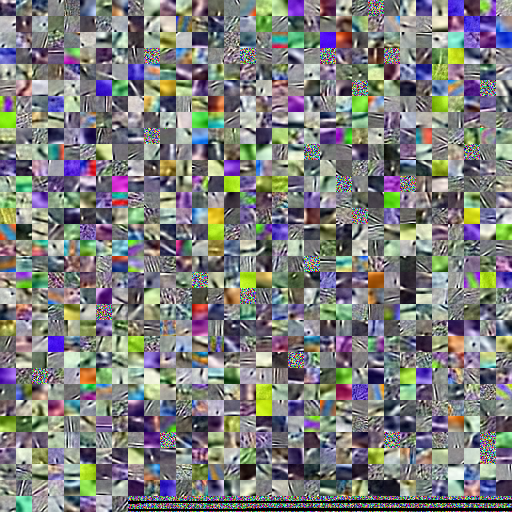
\includegraphics[width =
0.4\textwidth]{images/16_1000_1000_10_lasso.png}}
\hspace{5mm}
\subfloat[high pass]{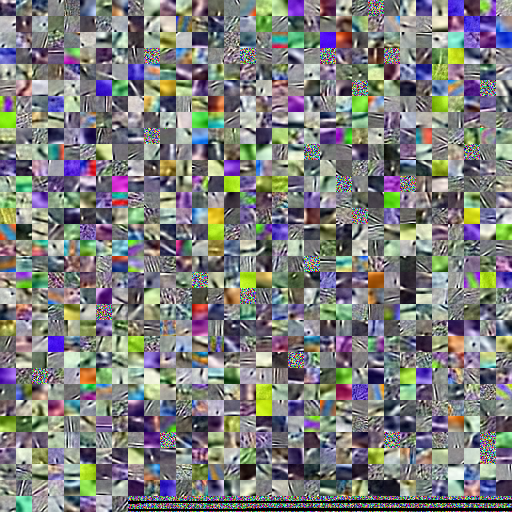
\includegraphics[width =
0.4\textwidth]{images/16_1000_1000_10_lasso.png}}
\caption{low pass}
\label{fig:16_1000_lasso}
\end{figure}
\begin{figure}
\centering
\subfloat[low pass]{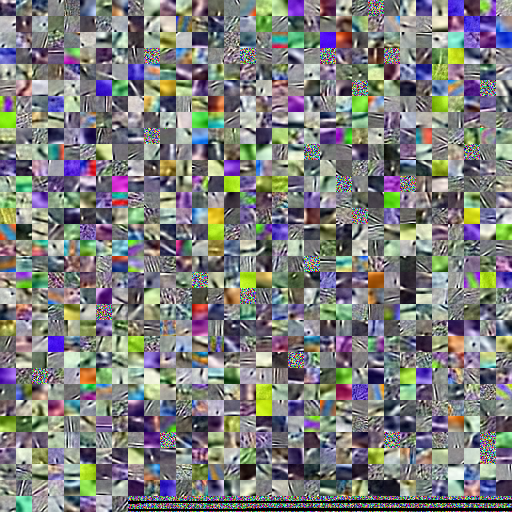
\includegraphics[width =
0.4\textwidth]{images/16_1000_1000_10_lasso.png}}
\hspace{5mm}
\subfloat[high pass]{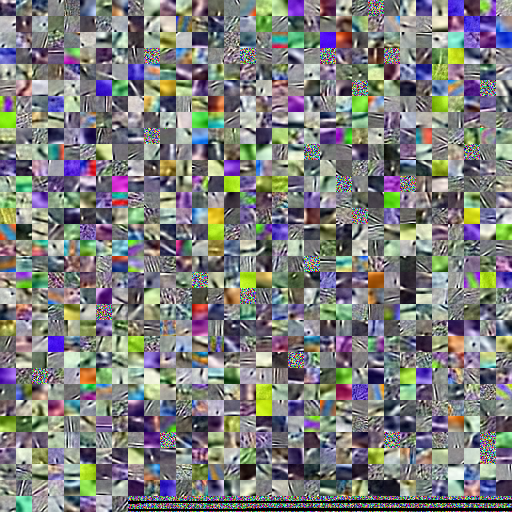
\includegraphics[width =
0.4\textwidth]{images/16_1000_1000_10_lasso.png}}
\caption{low pass}
\label{fig:16_1000_lasso}
\end{figure}
\begin{figure}
\centering
\subfloat[low pass]{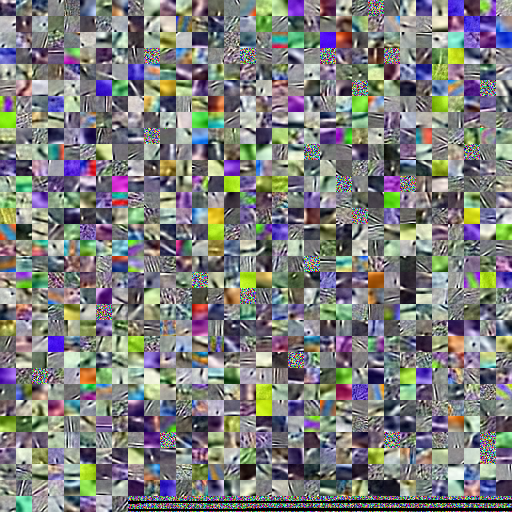
\includegraphics[width =
0.4\textwidth]{images/16_1000_1000_10_lasso.png}}
\hspace{5mm}
\subfloat[high pass]{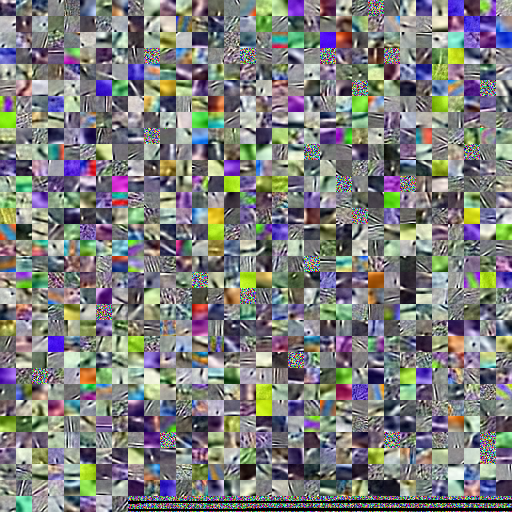
\includegraphics[width =
0.4\textwidth]{images/16_1000_1000_10_lasso.png}}
\caption{low pass}
\label{fig:16_1000_lasso}
\end{figure}

\section{Compression}

\subsection{Natural image database}


\begin{figure}[h]
\centering
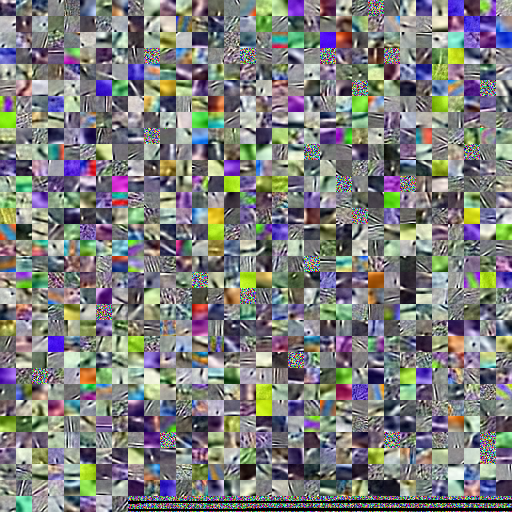
\includegraphics[width = 0.44\textwidth]{images/16_1000_1000_10_lasso.png}
\caption{16x16 LARS-lasso with 1000 elements}
\label{fig:16_1000_lasso}
\end{figure}

\begin{figure}
\centering
\subfloat[low pass]{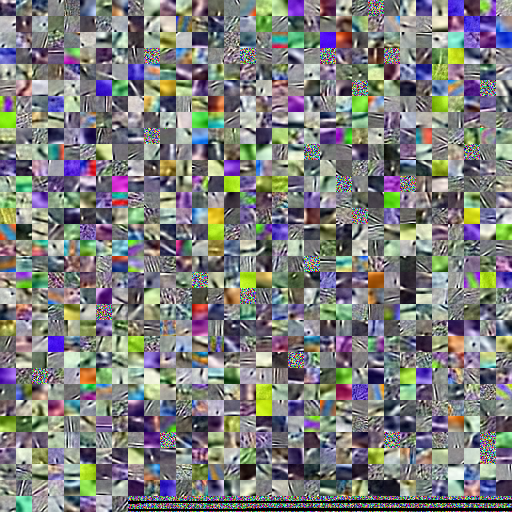
\includegraphics[width =
0.4\textwidth]{images/16_1000_1000_10_lasso.png}}
\hspace{5mm}
\subfloat[high pass]{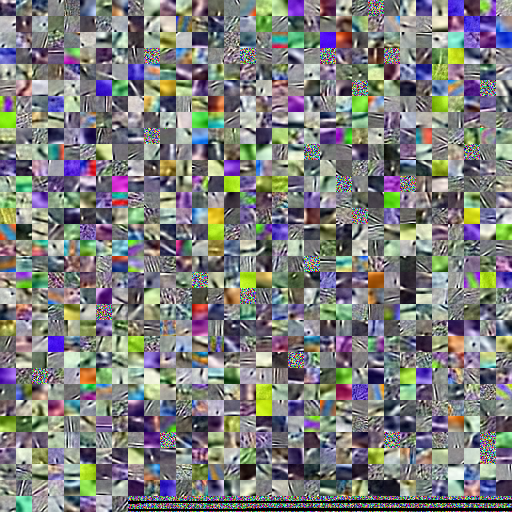
\includegraphics[width =
0.4\textwidth]{images/16_1000_1000_10_lasso.png}}
\caption{low pass}
\label{fig:16_1000_lasso}
\end{figure}
\begin{figure}
\centering
\subfloat[low pass]{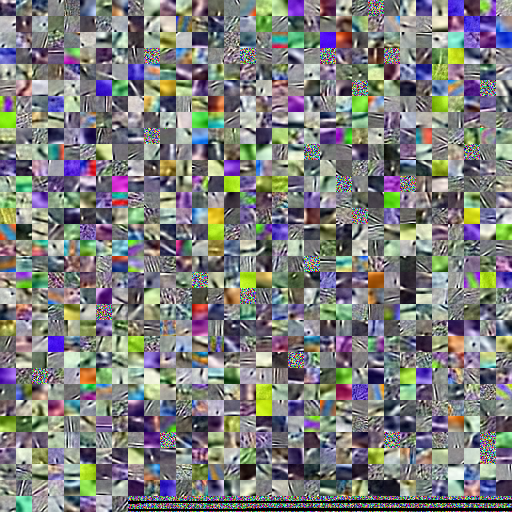
\includegraphics[width =
0.4\textwidth]{images/16_1000_1000_10_lasso.png}}
\hspace{5mm}
\subfloat[high pass]{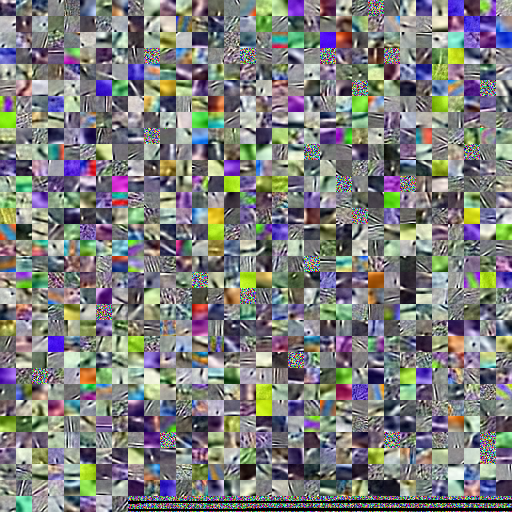
\includegraphics[width =
0.4\textwidth]{images/16_1000_1000_10_lasso.png}}
\caption{low pass}
\label{fig:16_1000_lasso}
\end{figure}
\begin{figure}
\centering
\subfloat[low pass]{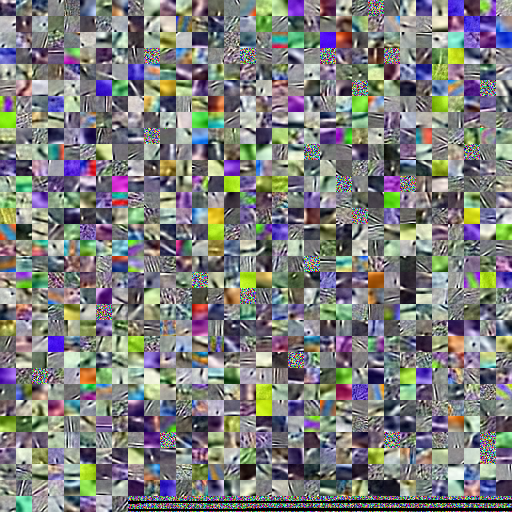
\includegraphics[width =
0.4\textwidth]{images/16_1000_1000_10_lasso.png}}
\hspace{5mm}
\subfloat[high pass]{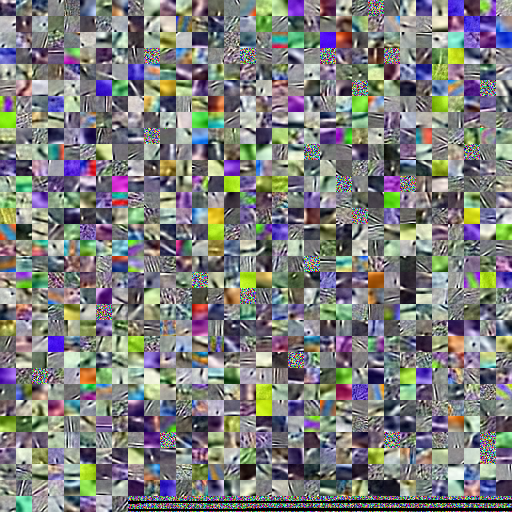
\includegraphics[width =
0.4\textwidth]{images/16_1000_1000_10_lasso.png}}
\caption{low pass}
\label{fig:16_1000_lasso}
\end{figure}



\subsection{Specific image groups}

\begin{figure}[h]
\centering

\includegraphics[width = 0.66\textwidth]{images/1000_sketches.png}
\caption{1000 16x16 elements of sketches database}
\label{fig:16_1000_lasso}
\end{figure}

\begin{figure}
\centering
\subfloat[low pass]{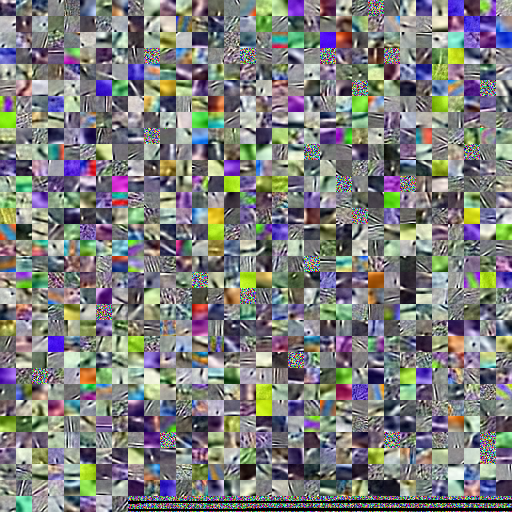
\includegraphics[width =
0.4\textwidth]{images/16_1000_1000_10_lasso.png}}
\hspace{5mm}
\subfloat[high pass]{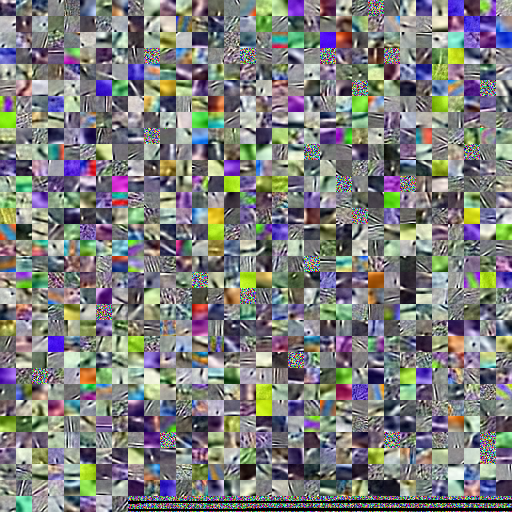
\includegraphics[width =
0.4\textwidth]{images/16_1000_1000_10_lasso.png}}
\caption{low pass}
\label{fig:16_1000_lasso}
\end{figure}
\begin{figure}
\centering
\subfloat[low pass]{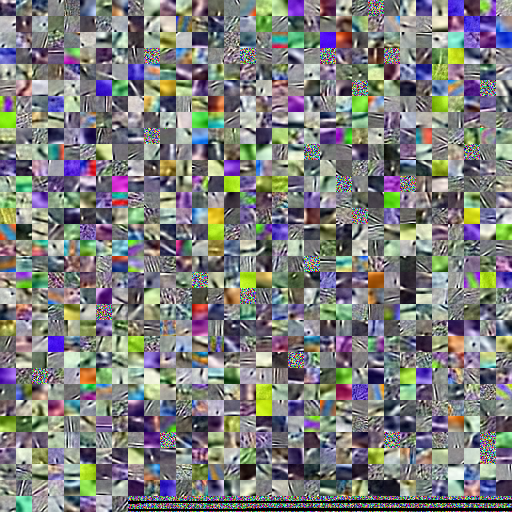
\includegraphics[width =
0.4\textwidth]{images/16_1000_1000_10_lasso.png}}
\hspace{5mm}
\subfloat[high pass]{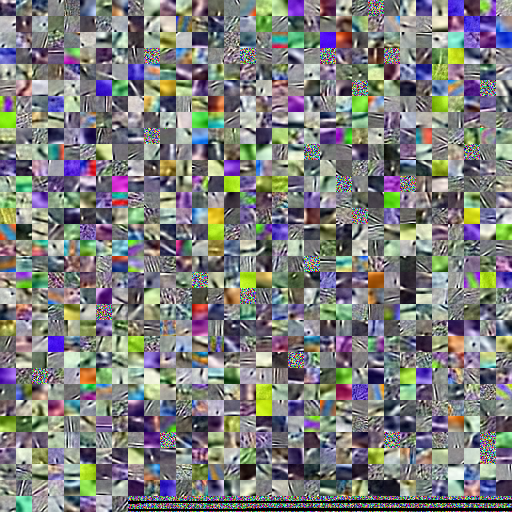
\includegraphics[width =
0.4\textwidth]{images/16_1000_1000_10_lasso.png}}
\caption{low pass}
\label{fig:16_1000_lasso}
\end{figure}
\begin{figure}
\centering
\subfloat[low pass]{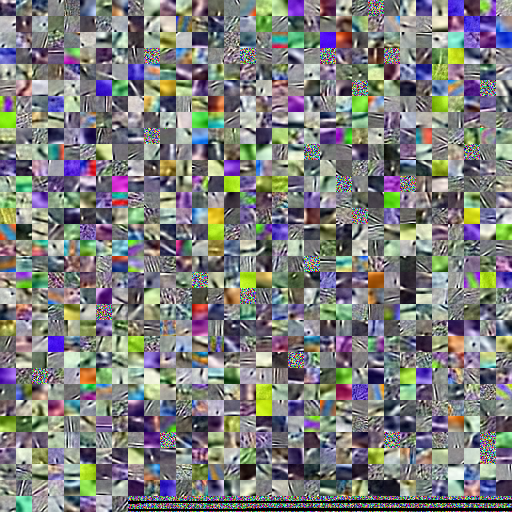
\includegraphics[width =
0.4\textwidth]{images/16_1000_1000_10_lasso.png}}
\hspace{5mm}
\subfloat[high pass]{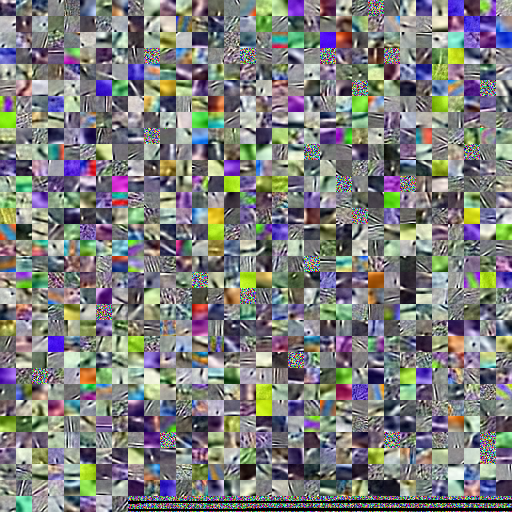
\includegraphics[width =
0.4\textwidth]{images/16_1000_1000_10_lasso.png}}
\caption{low pass}
\label{fig:16_1000_lasso}
\end{figure}
%\section{Quality}
%\subsection*{trained vs. analytical base}
%\subsection*{Compression ratio}
%\subsection*{Dictionary size}
%Setup:
%  initialize: random pixels, radom samples 
%  dict size: 256, 1000, 4000, 8000
%  coeffs: 5, 10, 20









